\chapter{Choices}

\section{Comparative statics}

Consumer maximization problem:
\begin{align*}
    \max & \ \text{Utility Function} \\
    \text{s.t.} & \ \text{Budget Constraint} \\
    \implies & \mathbf{x}^*(\mathbf{p}, m) \text{ is the optimal choice.}
\end{align*}

\block{Definition: Income Expension Path}{
Holding price constant and allow income to vary; 
the resulting locus of utility maximizing bundle is known as the \textbf{income expansion path}.
($\mathbf{p}$固定、$m$變動所形成最佳消費組合$\mathbf x$之連線。)
}

\block{Definition: Engle Curve}{
Derive from income expansion curve, it's a function that related to demand for each commodity.
}

\begin{enumerate}
    \item The income expansion path (and thus Engle curve) is a straight line through the origin.
    In this case the consumer is said to have demand curves with unit income elasticity. 
    Such a consumer will consume the same proportion of each commodity at each level of income.
    \begin{itemize}
        \item $\frac{\partial \mathbf{x}}{\partial m} = 0$
    \end{itemize}
    \item The income expansion path bends toward one good or the other, that is as consumer gets more income, he consumes more of both goods but proportionally more of one good (the luxury good) than of the other (the necessary good). 
    (收入增加需求佔比增加為奢侈品;收入增加需求佔比減少為必需品。)
    \begin{itemize}
        \item Luxury good: $\frac{\partial \mathbf{x}}{\partial m} > 1$
        \item Necessary good: $\frac{\partial \mathbf{x}}{\partial m} < 1$
    \end{itemize}
    \item If the income expansion path could bend backwards in this case and increase in income means the consumer actually wants to consume less of one of the good. Such goods are called inferior good;
    goods for which more income means more demand are called normal goods.
    (收入增加需求增加為普通財;收入增加需求減少為劣等財。)
    \begin{itemize}
        \item Normal good: $\frac{\partial \mathbf{x}}{\partial m} > 0$
        \item Inferior good: $\frac{\partial \mathbf{x}}{\partial m} < 0$
    \end{itemize}
\end{enumerate}

\begin{figure}[h]
    \center
    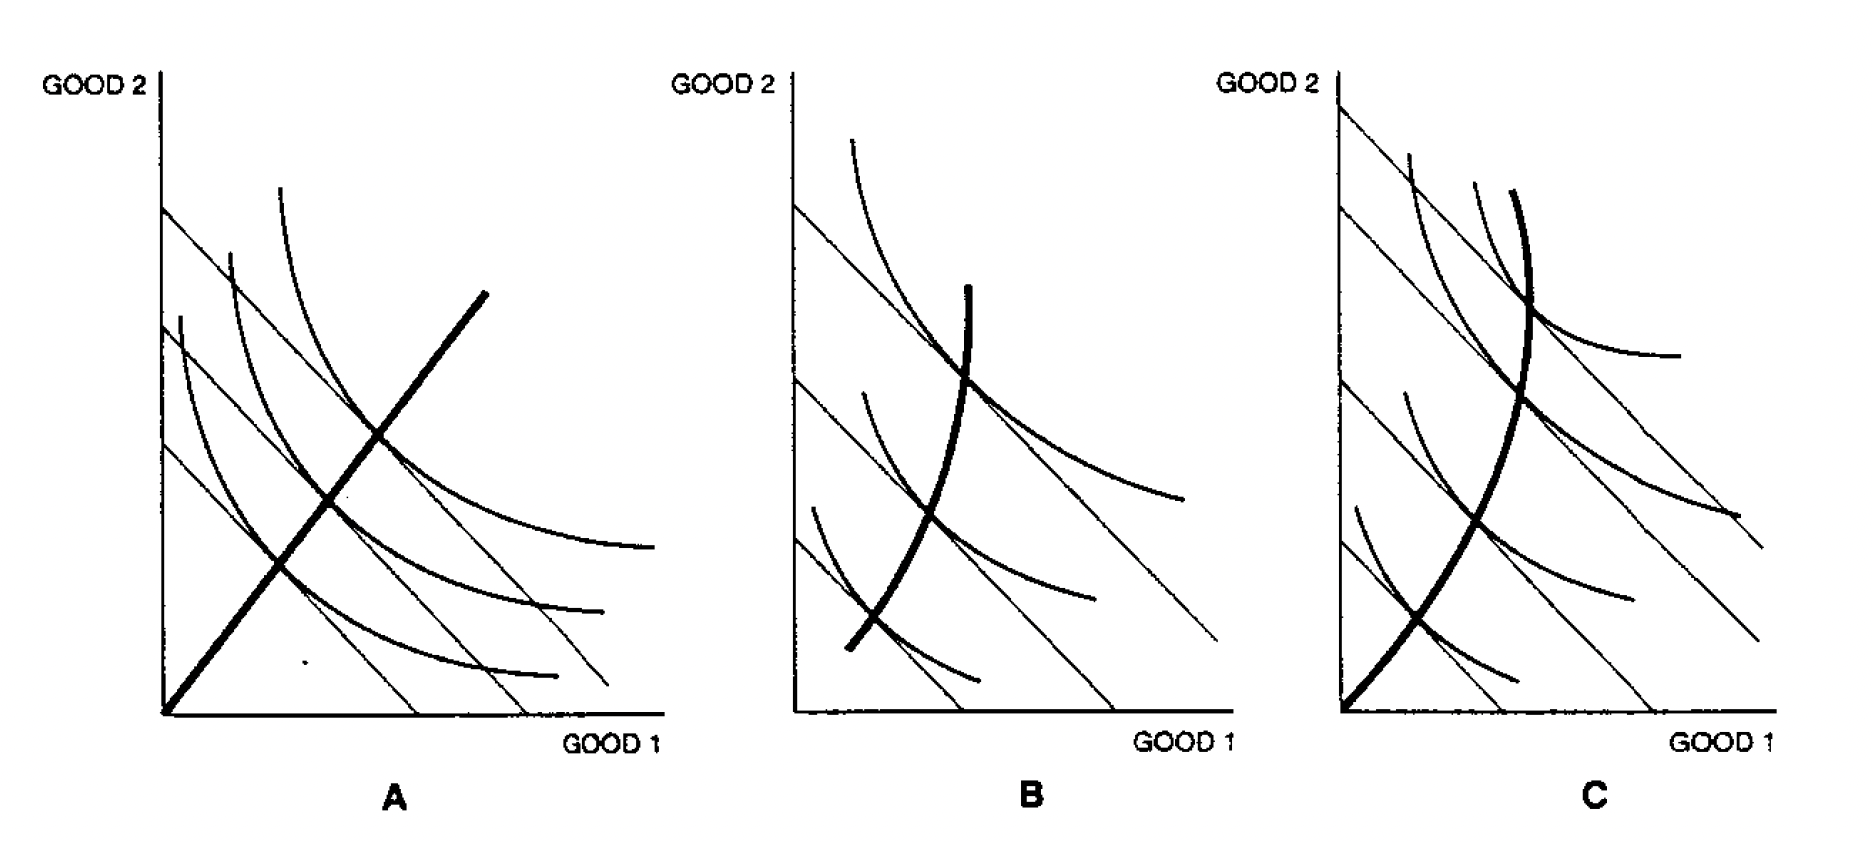
\includegraphics[width=0.7\textwidth]{img/fig8-1-1.png}
    \caption{}
\end{figure}

\block{Definition: Price Offer Curve}{
    Holding income fixed and allow prices to vary. If we let $p_1$ vary and hold $p_2$ and $m$ fixed, our budget line will tilt, and the locus of tangencies will sweep out a curve know as the \textbf{price offer curve}.
    ($m$固定、$\mathbf{p}$變動所形成最佳消費組合$\mathbf x$之連線。)
}

\begin{enumerate}
    \item In ordinary case, lower price for good 1 would lead to greater demand for the good.
    (價格減少需求增加,一般情況。)
    \begin{itemize}
        \item $\frac{\partial \mathbf{x}}{\partial p_i} < 0$
    \end{itemize}
    \item If we have a situation where a decrease in the price of good 1 brings about a decrease demand of good 1.
    Such a good is called \textbf{Giffen good}.
    (價格減少需求減少,季芬財。)
    \begin{itemize}
        \item $\frac{\partial \mathbf{x}}{\partial p_i} > 0$
    \end{itemize}
\end{enumerate}

\begin{figure}[h]
    \center
    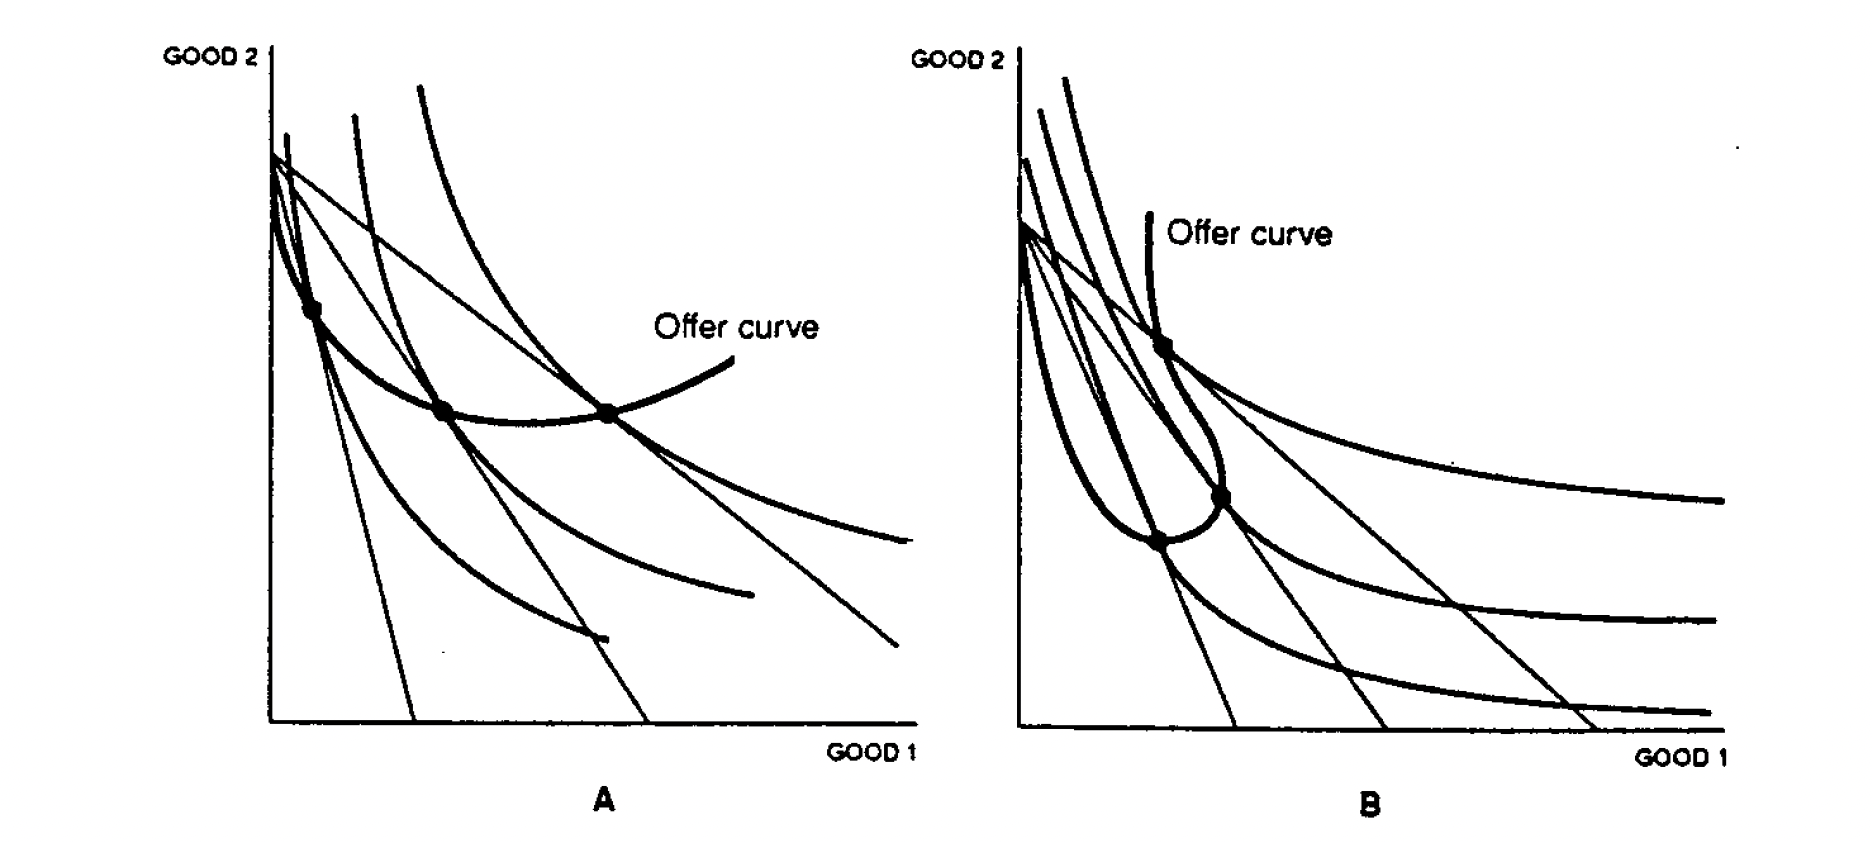
\includegraphics[width=0.7\textwidth]{img/fig8-2.png}
    \caption{}
\end{figure}

\block{Example: Excise and Income Taxes}{
    Initially,  consumers budget constraint is $p_1x_1 + p_2x_2 = m$.
    \begin{enumerate}
        \item \textbf{Excise tax}: \\
        After we impose a tax on sale of good 1 the budget constraint becomes 
        \[
            (p_1+t)x_1 + p_2x_2 = m.
        \]
        Suppose we let after tax level of consumption by $(x_1^*, x_2^*)$, then the revenue collected by the tax is $tx_1^*$.

        \item \textbf{Income tax}: \\
        Suppose now that we decide to collect the same amount of revenue by tax on income. The budget constraint of the consumer would then be 
        \[
            p_1x_1 + p_2x_2 = m-tx_1^*.
        \]
        This is a line with slope $-p_1/p_2$ that through the indifference curve at $(x_1^*, x_2^*)$.
    \end{enumerate}
    Therefore, A consumer is always worse off facing an excise tax than an income tax that generates the same revenue.
}
\begin{figure}[h]
    \center
    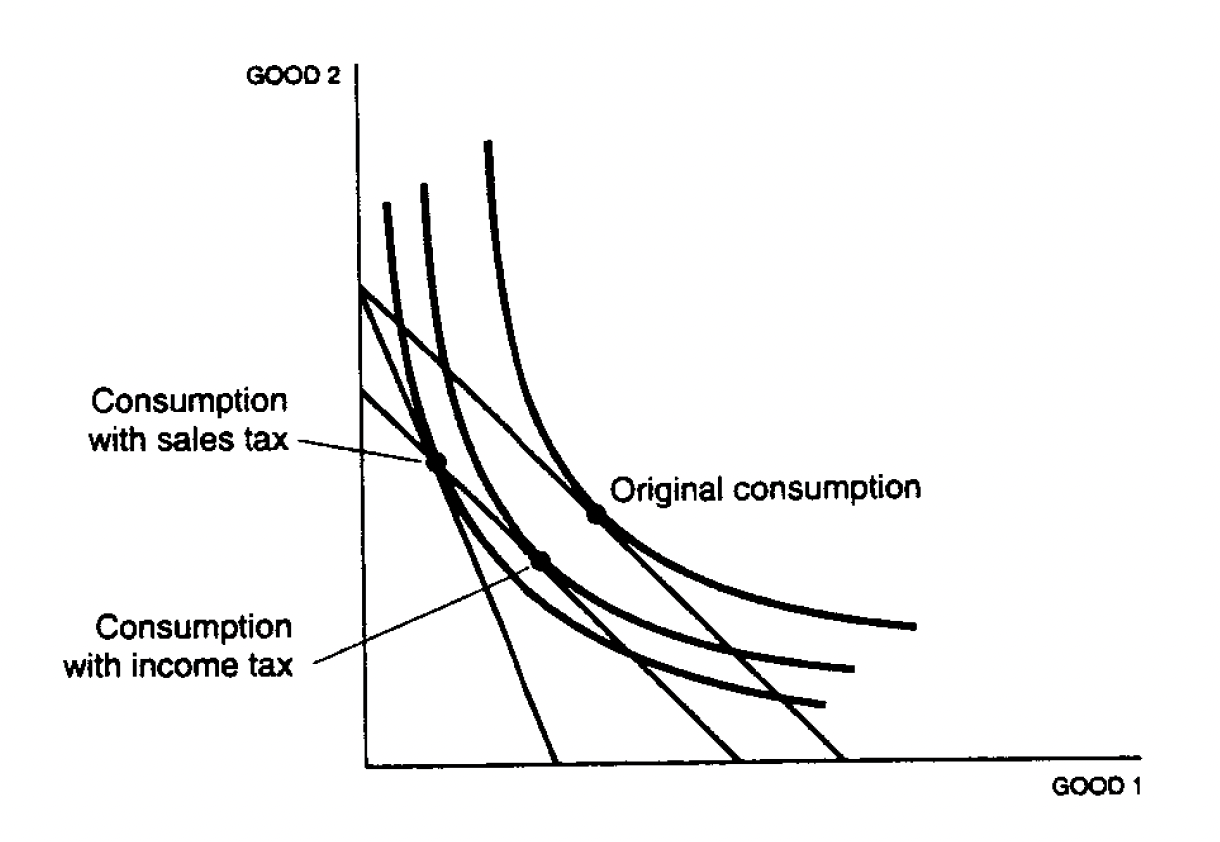
\includegraphics[width=0.7\textwidth]{img/fig8-3.png}
    \caption{}
\end{figure}

\section{The Slusky equation}

The Hicksian, or compensated demand curve, is formally the same as the conditional factor demand. It has all the same properties:
\begin{enumerate}
    \item HD-0
    \item Symmetric, negetive semidefinite  substitution matrix.
\end{enumerate}

\block{Theorem: Slusky equation}{
    \[
        \frac{\partial x_j (\mathbf p, m)}{\partial p_i} = 
        \frac{\partial h_j (\mathbf p, v(\mathbf p, m))}{\partial p_i} -
        \frac{\partial x_j (\mathbf p, m)}{\partial m} x_i (\mathbf p, m)
    \]
    \pf{
        Let $\mathbf x^*$  maximize utility at $(\mathbf p^*,m^*)$ and let  $u^* = u^*(\mathbf x^*)$. It is identically true that 

        \[
        h_j(\mathbf p^*, u^*) \equiv
        x_j(\mathbf p^*, e(\mathbf p^*, u^*)).
        \]

        We can differentiate this with respect to $p_i$ and evaluate the derivative at $\mathrm p^*$ to get 

        \[
        \frac{\partial h_j(\mathbf p^*, u^*) }{\partial p_i} 
        \equiv
        \frac{\partial x_j(\mathbf p^*, m^*) }{\partial p_i} 
        + 
        \frac{\partial x_j(\mathbf p^*, m^*) }{\partial m} \frac{\partial e(\mathbf p^*, u^*) }{\partial p_i}
        \]

        \begin{itemize}
            \item $\frac{\partial h_j(\mathbf p^*, u^*) }{\partial p_i}$ : how the compensated demand changes when $p_i$ changes.
            \item $\frac{\partial x_j(\mathbf p^*, m^*) }{\partial p_i}$ : the change in demand holding expenditure fixed at $m^*$.
            \item $\frac{\partial x_j(\mathbf p^*, m^*) }{\partial m}$ : the change in demand when income changes.
            \item $\frac{\partial e(\mathbf p^*, u^*) }{\partial p_i}$: how much income has to change to keep utility constant, is just $x_i^*$.
        \end{itemize}

        \[
        \implies
        \frac{\partial x_j(\mathbf p^*, m^*) }{\partial p_i} 
        =
        \frac{\partial h_j(\mathbf p^*, u^*) }{\partial p_i} 
        -
        \frac{\partial x_j(\mathbf p^*, m^*) }{\partial m} x_i^*,
        \]

        which is Slutsky equation.
    }
}
The Slutsky equation decomposes the demand change induced by a price change $\Delta p_i$ into two separate effects: the \textbf{substitution effect} and the \textbf{income effect}:
\[
    \Delta x_j \approx
    \frac{\partial x_j(\mathbf p, m) }{\partial p_i} \Delta p_i
    = \underbrace{
    \frac{\partial h_j(\mathbf p, u) }{\partial p_i} \Delta p_i}_{\text{substitution effect}}
    - \underbrace{
    \frac{\partial x_j(\mathbf p, m) }{\partial m} x_i \Delta p_i}_{\text{income effect}}.
\]
General form of Slutsky equation
\begin{align*}
    \mathbf D_p \mathbf x(\mathbf p, m)
    &=
    \mathbf D_p \mathbf h(\mathbf p, u)
    -
    \mathbf D_m \mathbf x(\mathbf p, m) \mathbf x\\
    \begin{bmatrix}
    \frac{\partial x_1(\mathbf p, u) }{\partial p_1} &
    \frac{\partial x_1(\mathbf p, u) }{\partial p_2} \\
    \frac{\partial x_2(\mathbf p, u) }{\partial p_1} &
    \frac{\partial x_2(\mathbf p, u) }{\partial p_2}
    \end{bmatrix}
    &=
    \begin{bmatrix}
    \frac{\partial h_1(\mathbf p, m) }{\partial p_1} &
    \frac{\partial h_1(\mathbf p, m) }{\partial p_2} \\
    \frac{\partial h_2(\mathbf p, m) }{\partial p_1} &
    \frac{\partial h_2(\mathbf p, m) }{\partial p_2}
    \end{bmatrix}
    -
    \begin{bmatrix}
    \frac{\partial x_1(\mathbf p, m) }{\partial m} \\
    \frac{\partial x_2(\mathbf p, m) }{\partial m} 
    \end{bmatrix}
    \begin{bmatrix}
    x_1 & x_2
    \end{bmatrix}
    \\
    &=
    \begin{bmatrix}
    \frac{\partial h_1(\mathbf p, m) }{\partial p_1} &
    \frac{\partial h_1(\mathbf p, m) }{\partial p_2} \\
    \frac{\partial h_2(\mathbf p, m) }{\partial p_1} &
    \frac{\partial h_2(\mathbf p, m) }{\partial p_2}
    \end{bmatrix}
    -
    \begin{bmatrix}
    \frac{\partial x_1(\mathbf p, m) }{\partial m} x_1 &
    \frac{\partial x_1(\mathbf p, m) }{\partial m} x_2\\
    \frac{\partial x_2(\mathbf p, m) }{\partial m} x_1 &
    \frac{\partial x_2(\mathbf p, m) }{\partial m} x_2
    \end{bmatrix}.
\end{align*}
Let $\Delta \mathbf p =(\Delta p_1, \Delta p_2), \ \Delta \mathbf x =(\Delta x_1, \Delta x_2)$,
\begin{align*}
    \begin{bmatrix}
        \Delta x_1 \\ \Delta x_2
    \end{bmatrix}
    &\approx
    \underbrace{
    \begin{bmatrix}
    \frac{\partial h_1}{\partial p_1} &
    \frac{\partial h_1}{\partial p_2} \\
    \frac{\partial h_2}{\partial p_1} &
    \frac{\partial h_2}{\partial p_2}
    \end{bmatrix}
    \begin{bmatrix}
    \Delta p_1 \\ \Delta p_2
    \end{bmatrix}
    }_{\text{substitution effect}}
    - \underbrace{
    \begin{bmatrix}
    \frac{\partial x_1}{\partial m} x_1 &
    \frac{\partial x_1}{\partial m} x_2\\
    \frac{\partial x_2}{\partial m} x_1 &
    \frac{\partial x_2}{\partial m} x_2
    \end{bmatrix}
    \begin{bmatrix}
    \Delta p_1 \\ \Delta p_2
    \end{bmatrix}
    }_{\text{income effect}}
    \\
    &=
    \begin{bmatrix}
    \Delta x_1^s \\ \Delta x_2^s
    \end{bmatrix}
    -
    \begin{bmatrix}
    \Delta x_1^m \\ \Delta x_2^m
    \end{bmatrix}
\end{align*}

\begin{itemize}
    \item Substitution effect: indicate how the Hicksian demand change, it change along indifference curve.
    \item Income effect: indicate the impact of this change on demand, with prices hheld constant at the initial level. (Therefore, the vector lies along the income expansion path.)
\end{itemize}

\begin{figure}[h]
    \center
    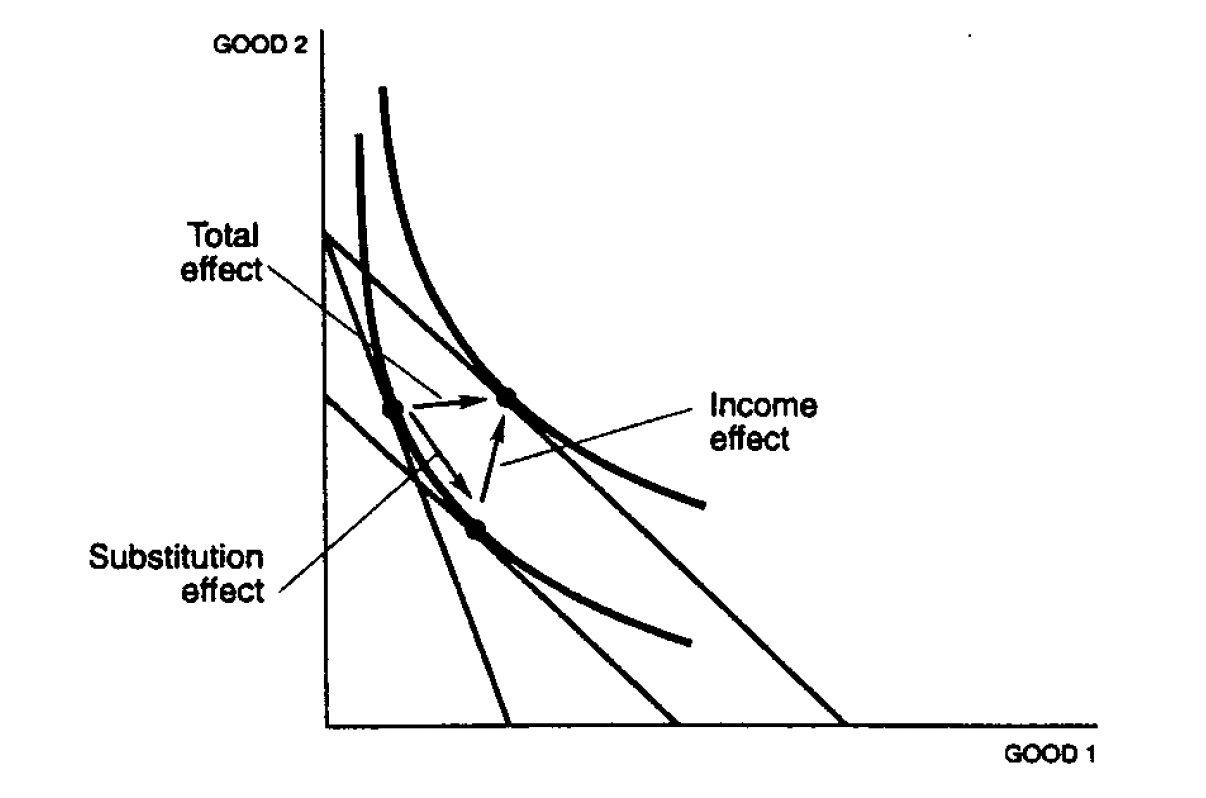
\includegraphics[width=0.7\textwidth]{img/fig8-4.png}
    \caption{}
\end{figure}

\block{Example: The Cobb-Douglas Slutsky Equation}{
    Since $u = x_1^{\alpha-1}x_2^{1-\alpha}$, we have
    \begin{align*}
        v(p_1, p_2, m) &= mp_1^{-a} p_2^{a-1} \\
        e(p_1, p_2, u) &= up_1^{a} p_2^{1-a} \\
        x_1(p_1, p_2, m) &= \frac{am}{p_1} \\
        h_1(p_1, p_2, u) &= \frac{\partial e}{\partial p_1} = ap_1^{a-1} p_2^{1-a} u %\\
        % x_2(p_1, p_2, m) &= \frac{(1-a)m}{p_2} \\
        % h_2(p_1, p_2, u) &= \frac{\partial e}{\partial p_2} = .
    \end{align*}
    Thus, 
    \begin{align*}
        \frac{\partial x_1(\mathbf{p}, m)}{\partial p_1} &= -\frac{am}{p_1^2} \\
        \frac{\partial x_1(\mathbf{p}, m)}{\partial m} &= \frac{a}{p_1} \\
        \frac{\partial h_1(\mathbf p, u)}{\partial p_1} &= a(a-1)p_1^{a-2} p_2^{1-a} u \\
        \frac{\partial h_1(\mathbf p, v(\mathbf p, m))}{\partial p_1} &= a(a-1)p_1^{a-2} p_2^{1-a} (mp_1^{-a} p_2^{a-1}) \\
        &= a(a-1)p_1^{-2}m.
    \end{align*}
    Now plug into the Slutsky equation to find
    \begin{align*}
        \frac{\partial h_1}{\partial p_1}-
        \frac{\partial x_1}{\partial m} x_1 &= 
        \frac{a(a-1)m}{p_1^{-2}} - 
        \frac{a}{p_1}\frac{am}{p_1} \\
        &=\frac{-am}{p_1^2}
        =\frac{\partial x_1}{\partial p_1}
    \end{align*}
}

 
\section{Properties of demand functions}

\block{Theorem: Neoclassical Theory of Consumer Behavior}{
    \begin{enumerate}
        \item (負定) The matrix of substitution terms $\frac{\partial h_j(\mathbf p, u)}{\partial p_i}$ is negative semi-definite because the expenditure function is concave
    
        \[
            \frac{\partial h_j(\mathbf p, u)}{\partial p_i} = 
            \frac{\partial [\frac{\partial e(\mathbf p, u)}{\partial p_j}]}{\partial p_i} = 
            \frac{\partial^2 e(\mathbf p, u)}{\partial p_i \partial p_j}
        \]
        
        \item (對稱) The matrix of substitution terms is symmetric
            
        \[
            \frac{\partial h_j(\mathbf p, u)}{\partial p_i} = 
            \frac{\partial^2 e(\mathbf p, u)}{\partial p_i \partial p_j}= 
            \frac{\partial^2 e(\mathbf p, u)}{\partial p_j \partial p_i}=
            \frac{\partial h_i(\mathbf p, u)}{\partial p_j}
        \]
            
        \item (對角向為負) In particular, “the compensated own-price effect is nonpositive”; that is, the Hicksian demand curve slope downward:
            
            \[
            \frac{\partial h_i(\mathbf p, u)}{\partial p_i} = 
            \frac{\partial^2 e(\mathbf p, u)}{\partial p_i^2} \leq 0
            \]
            
            Since the substitution matrix is negative semi-definite and thus ha non-positive diagonal terms.
            
        \item (替代矩陣負定且對稱) The substitution matrix $(\frac{\partial x_j(\mathbf p, u) }{\partial p_i} + \frac{\partial x_j(\mathbf p, m) }{\partial m} x_i)$ is a symmetric, negative semi-definite matrix.
    \end{enumerate}
}


\section{Comparative statics using the first order condition}

The first order condition of the utility maximization problem gives us:
\begin{align*}
    p_1 x_1(p_1, p_2, m) +p_2 x_2(p_1, p_2, m)-m \equiv 0 \\
    \frac{\partial u( x_1(p_1, p_2, m) , x_2(p_1, p_2, m))}{\partial x_1} -\lambda p_1 \equiv 0 \\
    \frac{\partial u( x_1(p_1, p_2, m) , x_2(p_1, p_2, m))}{\partial x_2} -\lambda p_2 \equiv 0.
\end{align*}

\subsection*{Substitution effect}

Differenting with respect to $p_1$, and arraging in matrix form, we have
\begin{align*}
    \begin{bmatrix}
        0 & -p_1 &-p_2 \\
        -p_1 & u_{11} & u_{12} \\
        -p_2 & u_{21} & u_{22}
    \end{bmatrix}
    \begin{bmatrix}
        \frac{\partial \lambda}{\partial p_1} \\
        \frac{\partial x_1}{\partial p_1}\\
        \frac{\partial x_2}{\partial p_1}
    \end{bmatrix}
    \equiv
    \begin{bmatrix}
        x_1 \\
        \lambda \\
        0
    \end{bmatrix}.
\end{align*}
Using Cramer's rule, 
\[
    \frac{\partial x_1}{\partial p_1} = 
    \frac{
    \begin{vmatrix}
    0 & x_1 &-p_2 \\
    -p_1 & \lambda & u_{12} \\
    -p_2 &0 & u_{22}
    \end{vmatrix}
    }{H}
    =
    \frac{\lambda
    \begin{vmatrix}
    0 & -p_2 \\
    -p_2 & u_{22}
    \end{vmatrix}
    }{H}
    -
    \frac{x_1
    \begin{vmatrix}
    -p_1 & u_{12} \\
    -p_2 & u_{22}
    \end{vmatrix}
    }{H}
\]
\subsection*{Income effect}

Differentiating with respect to $m$.
\[
    \begin{bmatrix}
        0 & -p_1 &-p_2 \\
        -p_1 & u_{11} & u_{12} \\
        -p_2 & u_{21} & u_{22}
        \end{bmatrix}
        \begin{bmatrix}
        \frac{\partial \lambda}{\partial p_1} \\
        \frac{\partial x_1}{\partial p_1}\\
        \frac{\partial x_2}{\partial p_1}
        \end{bmatrix}
        \equiv
        \begin{bmatrix}
        -1 \\
        0 \\
        0
    \end{bmatrix}.
\]
By Cramer's rule,
\[
    \frac{\partial x_1}{\partial m} = 
    \frac{
    \begin{bmatrix}
    0 & -p_1 &-1 \\
    -p_1 & u_{11} & 0 \\
    -p_2 & u_{21} & 0
    \end{bmatrix}
    }{H}
    =
    \frac{
    \begin{vmatrix}
    -p_1 & u_{12} \\
    -p_2 & u_{22}
    \end{vmatrix}
    }{H}.
\] 
\section{The integrability problem}
Skip.

\section{Duality in consumption}
\[
    \begin{array}{r l}
        v(\mathbf{p}) = \max & \ u(\mathbf{x}) \\
        \text{s.t.} & \ \mathbf{px} = 1 
    \end{array}
    \iff
    \begin{array}{r l}
        u(\mathbf{x}) = \min & \ v(\mathbf{p}) \\
        \text{s.t.} & \ \mathbf{px} = 1 
    \end{array}
\]

\block{Example: Solving for the direct utility function}{
    Indirect utility function: $v(p_1, p_2)= -a \ln p_1 -b \ln p_2$.
    The minimization problem:
    \begin{align*}
        \underset{p_1, p_2}{\min} & \ -a \ln p_1 -b \ln p_2 \\
        \text{s.t.} & \ 
        p_1x_1+p_2x_2 = 1 \\
        \implies \mathcal{L} =& -a \ln p_1 -b \ln p_2 - \lambda(p_1x_1+p_2x_2 - 1)
    \end{align*}
    The FOCs are:
    \begin{align*}
        \begin{cases}
            -a /p_1 = \lambda x_1 \\
            -b /p_2 = \lambda x_2 \\
            p_1x_1+p_2x_2 = 1
        \end{cases}
        &\implies
        \begin{cases}
        -a = \lambda x_1 p_1\\
        -b = \lambda x_2 p_2\\
        p_1x_1+p_2x_2 = 1
        \end{cases}
        \\
        &\implies
        \begin{cases}
        -a = \lambda x_1 p_1\\
        -b = \lambda x_2 p_2\\
        (p_1x_1+p_2x_2)\lambda = \lambda
        \end{cases}
        \\
        &\implies -a-b=\lambda
    \end{align*}
    Substitute back to the FOCs to find the inverse demand:
    \[
        \implies
        \begin{cases}
        p_1 = \frac{a}{(a+b)x_1} \\
        p_2 = \frac{b}{(a+b)x_2}
        \end{cases}
    \]
    Substitute the choices of $(p_1, p_2)$ into the indirect utility function:
    \begin{align*}
        u(x_1, x_2)
        =& -a \ln p_1 -b \ln p_2 \\
        =& 
        -a \ln \frac{a}{(a+b)x_1} 
        -b \ln \frac{b}{(a+b)x_2} \\
        =&
        -a(\ln a - \ln(a+b)-\ln x_1)
        -b(\ln b - \ln(a+b)-\ln x_2) \\
        =&
        a \ln x_1 +b \ln x_2
        -a\ln a -b\ln b 
        +(a+b)\ln(a+b) \\
        =&
        a \ln x_1 +b \ln x_2+\text{constant}.
    \end{align*}
    This is Cobb-Douglas utility function.
}

\section{}
Skip
\section{}
Skip


\section{Comparative statics using revealed preference}

\block{Definition: Hicksian Compensation}{
    The demand for the good in question if we change the level of income so as to restore the original level of utility $u$. 
    When $\mathbf p \to \mathbf p + \Delta \mathbf p$,
    \[
        x_i(\mathbf p+ \Delta \mathbf p, m+ \Delta m) \equiv x_i[\mathbf p+ \Delta \mathbf p, e(\mathbf p+ \Delta \mathbf p, u)]
    \]
    (當價格改變,所得要改變多少,使得在新價格之下,可以維持原來的效用水準。需要了解偏好、價格與消費組合。)
}

\block{Definition: Slutsky Compensation}{
    It is the level of demand that arises when income is changed so as to make the original level of consumption possible.
    \begin{align*}
        (\mathbf p+ \Delta \mathbf p) \mathbf{x}( \mathbf p , m) =  m + \Delta m \\
        \implies \Delta \mathbf p \ \mathbf x ( \mathbf{p} , m) = \Delta m
    \end{align*}
    (當價格改變,所得要改變多少,使得在新價格之下,負擔得起原來的消費組合。不需要了解偏好,只要知道價格與消費組合即可。)
}

\begin{figure}[h]
    \center
    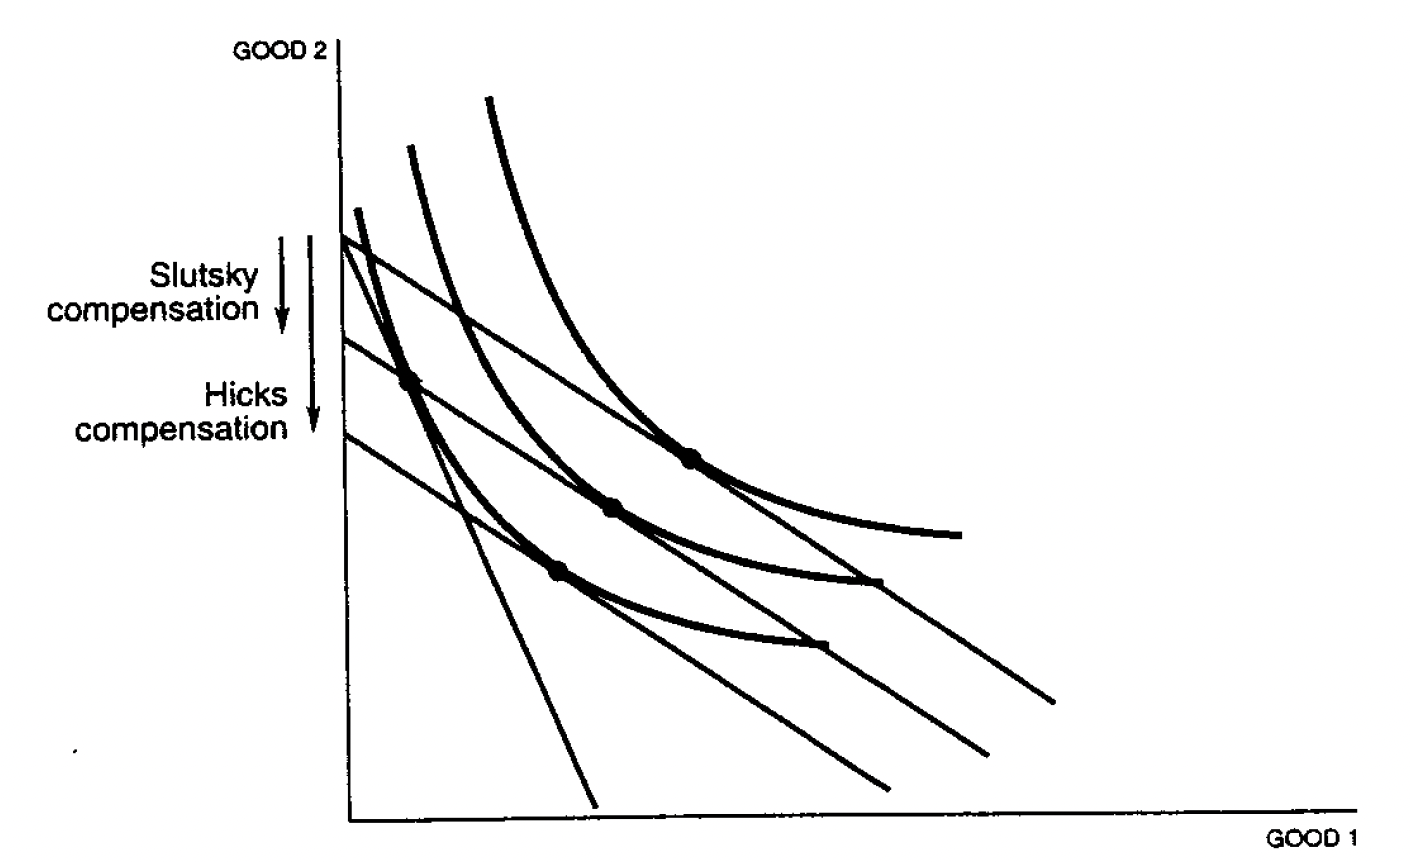
\includegraphics[width=0.7\textwidth]{img/fig8-6.png}
    \caption{}
\end{figure}

\section{}
Skip
\section{}
Skip